\documentclass[a4paper,12pt]{article}
\usepackage[numbers]{natbib}
\usepackage{graphicx}
\usepackage{amsmath, amssymb}
\usepackage[utf8]{inputenc}
\usepackage[T1]{fontenc}
% \usepackage{mathptmx} % Disabled: use default LaTeX Computer Modern font
\usepackage{geometry}
\usepackage{setspace}
\usepackage{float}
\usepackage{algorithm}
\usepackage{algpseudocode}
\usepackage{mdframed}
\usepackage{tikz}
\usepackage{enumitem}
\usepackage{xcolor}
\usepackage{colortbl}
\usepackage{placeins}
\usepackage{booktabs}
\usepackage{longtable}
\usepackage{array}
\usepackage{enumitem}
\usepackage{hyperref}


\usetikzlibrary{positioning, arrows.meta, shapes.geometric, fit, calc}
\geometry{top=2cm, bottom=2cm, left=2cm, right=2cm}
\onehalfspacing

\begin{document}

\begin{center}
    {\LARGE \textbf{Hanoi University of Science and Technology}}\\
    {\LARGE {School of Information and Communications Technology}}\\[0.8cm]
    \includegraphics[width=0.45\textwidth]{logo-soict-hust-1 (1).png}\\[1cm]
\end{center}

\begin{center}
    {\LARGE \textbf{
}\\[0.2cm]
    {\LARGE \textbf{PROJECT REPORT}\\[0.2cm]
    }
    }
\end{center}

\begin{center}
\begin{tabular}{p{0.45\textwidth} p{0.45\textwidth}}
    \begin{center}
        \textbf{Ninh Minh Hieu}\\
        Data Science \& AI\\
        HUST\\
        \texttt{Hieu.nm2416688@hust.sis.edu.vn}
    \end{center}
    &
    \begin{center}
        \textbf{Hoang Bao Huy}\\
        Data Science \& AI\\
        HUST\\
        \texttt{Huy.hb16705@sis.hust.edu.vn}
    \end{center}
\end{tabular}
\begin{tabular}{p{0.45\textwidth} p{0.45\textwidth}}
    \begin{center}
        \textbf{Nguyen Cong Hung}\\
        Data Science \& AI\\
        HUST\\
        \texttt{hung.nc2416702@sis.hust.edu.vn}
    \end{center}
    &
    \begin{center}
        \textbf{Nguyen Hoang Quan}\\
        Data Science \& AI\\
        HUST\\
        \texttt{Quan.nh2416738@sis.hust.edu.vn}
    \end{center}
\end{tabular}
\vspace{1cm}
\begin{center}
        \textbf{Le The Quyen}\\
        Data Science \& AI\\
        HUST\\
        \texttt{Quyen.lt2416743@sis.hust.edu.vn}
    \end{center}

\vspace{0.5cm}

\end{center}

\begin{center}
    \begin{tabular}{ll}
        \textbf{Course:} & Machine Learning
 \\
        \textbf{Class ID:} & 168272 \\
        \textbf{Semester:} & 20252 \\
        \textbf{Supervisor:} & Dr.\ Dam Quang Tuan \\
    \end{tabular}
\end{center}

\vfill

\begin{center}
    \textbf{Hanoi, 2026}
\end{center}

\tableofcontents
\newpage


\section*{Group Introduction}
\addcontentsline{toc}{section}{Group Introduction}
This report was prepared as a group project for the Machine Learning course. The project investigates bird and wildlife sound recognition from natural audio recordings using the BirdCLEF dataset. Since the project is developed by multiple members, the report covers several complementary directions: dataset analysis, audio preprocessing, spectrogram-based classification, sound event detection, class imbalance handling, semi-supervised learning, teacher-student training, self-distillation, and ensemble inference. The goal is not only to implement one isolated model, but to study how different machine learning components contribute to a practical bioacoustic recognition pipeline.

\section{Introduction}

\subsection{Dataset Background}
Bioacoustic monitoring is an important tool for studying biodiversity, ecological change, and species distribution in natural environments. Instead of relying only on visual observation, passive acoustic monitoring records environmental soundscapes and allows researchers to detect species from their vocalizations. Bird sound recognition is a representative problem in this field because many bird species have distinctive calls, songs, chirps, trills, and frequency-modulated patterns.

In this project, we use the BirdCLEF 2025 dataset as the main benchmark for studying bird and wildlife sound classification. The task is to estimate the presence probability of each target class from audio recordings. This setting is challenging because real-world recordings are noisy, labels may be incomplete, multiple species can vocalize in the same clip, and the distribution of species is highly imbalanced. In addition, there is a domain gap between directed recordings, which often focus on a single target species, and passive soundscape recordings, which are longer and contain richer background noise.

From a machine learning perspective, this task is naturally formulated as a multi-label audio classification problem. Each audio segment may contain zero, one, or multiple target species. Therefore, the model must output independent probabilities for all classes rather than using a single softmax prediction. This motivates the use of spectrogram-based convolutional networks, sound event detection, BCE-based training losses, semi-supervised learning, and ensemble inference.

\subsection{Project Objectives}
Our group studies a complete spectrogram-centered pipeline for bird sound recognition. The main objectives are:
\begin{itemize}
    \item to analyze the BirdCLEF dataset and identify the main modeling challenges, including class imbalance, multi-label annotations, domain shift, and unlabeled soundscape data;
    \item to build a spectrogram-based convolutional baseline using EfficientNet-family backbones;
    \item to extend the baseline into a sound event detection model that preserves temporal information and uses attention pooling;
    \item to investigate imbalance-aware training using sampling, class weighting, focal loss, and label smoothing;
    \item to study semi-supervised approaches, including pseudo-labeling, Noisy Student training, and self-distillation;
    \item to evaluate ensemble-based inference strategies, including multi-checkpoint averaging, shifted-window inference, and temporal smoothing.
\end{itemize}

\subsection{Report Organization}
The remainder of this report is organized as follows. Section 2 introduces the dataset and the exploratory analysis. Section 3 describes the preprocessing pipeline. Section 4 presents the model architecture, including the spectrogram classifier, EfficientNet backbone, SED formulation, and attention pooling. Section 5 discusses training strategies and loss functions. Section 6 presents semi-supervised and teacher-student methods. Section 7 describes inference and post-processing. Section 8 reports experimental results and ablation analysis. Sections 9 and 10 provide discussion and conclusion.

\section{Dataset and Exploratory Analysis}

\subsection{Dataset Overview}
We use the BirdCLEF 2025 dataset for our internal method study. The training set contains a total of $28{,}564$ audio samples, corresponding to approximately $280.5$ hours of audio recordings.

The test data consists of one-minute soundscape recordings collected through passive acoustic monitoring. All recordings are provided in Ogg format and resampled to $32$ kHz. The prediction setting is to estimate the probability of presence for each of the $206$ target classes in every five-second chunk of each audio file.

The training recordings come from three major sources: Xeno-Canto, iNaturalist, and the CSA collection provided by the Instituto Humboldt. Table~\ref{tab:samples-by-source} shows the number of samples from each source.

\begin{table}[htbp]
\centering
\caption{Number of training samples by data source.}
\label{tab:samples-by-source}
\begin{tabular}{lr}
\toprule
\textbf{Source} & \textbf{Number of samples} \\
\midrule
Xeno-Canto & $21{,}204$ \\
iNaturalist & $7{,}198$ \\
Other/CSA & $162$ \\
\bottomrule
\end{tabular}
\end{table}

In addition to primary labels, the metadata also includes secondary labels that describe background species appearing in the recordings. These labels are important because the test soundscapes may contain multiple species at the same time. In our dataset analysis, secondary species information appears in $4{,}958$ recordings, and the secondary-label field is available for $28{,}539$ recordings, which is approximately $99.9\%$ of the training data. This information can be used to better model the multi-label structure of the test set.

\subsection{Challenges}
\subsubsection{Class Imbalance}
The dataset has severe class imbalance, which is expected in ecological audio data because some species are naturally much rarer than others and therefore have fewer available recordings. In our dataset, the most common species is \texttt{grekis} with $990$ samples, while the rarest species, \texttt{64862}, has only $2$ samples. This gives an imbalance ratio of approximately $495\times$. There are $39$ species with fewer than $10$ samples, while only $9$ species have more than $500$ samples.

\begin{figure}[htbp]
\centering
\includegraphics[width=0.95\linewidth]{speciesDistribution.png}
\caption{Distribution of animal classes in the BirdCLEF 2025 training dataset.}
\label{fig:species-distribution}
\end{figure}

This imbalance is a major modeling problem. If the model is trained naively, it may learn to prioritize frequent species and ignore rare species. Therefore, we need to address class imbalance using techniques such as class-balanced sampling, loss reweighting, data augmentation, and careful validation.

\subsubsection{Multi-Label Nature}
One recording may contain multiple bird species simultaneously, such as crow, robin, and sparrow. The presence of secondary labels confirms that many recordings contain background species in addition to the primary target species. This means the problem should be treated as multi-label classification rather than single-label classification.

\subsubsection{Domain Shift Between Recordings}
There is a significant domain shift between passive acoustic monitoring soundscapes and directed recordings from sources such as Xeno-Canto. Directed recordings often focus on a target bird and may have clearer vocalizations, while soundscapes are longer, noisier, and contain more overlapping environmental sounds. However, some species that are underrepresented in the labeled training dataset may appear frequently in soundscape data. This creates an additional challenge, but it also motivates the use of semi-supervised learning and pseudo labeling.

\subsubsection{Unlabeled Data}
Unlabeled soundscape data provides an opportunity for pseudo labeling and other semi-supervised learning techniques. If used carefully, these recordings can reduce data loss and help the model adapt to the test-domain soundscape distribution.

\section{Data Preprocessing}

\subsection{Audio Segmentation}

Audio segmentation is an important preprocessing step because the BirdCLEF prediction setting requires predictions at a fixed temporal resolution. The dataset contains recordings with different durations: many soundscape recordings are close to one minute long, while some directed recordings are shorter than five seconds. Since our model is designed to predict bird presence on five-second audio segments, all input audio must be converted into fixed-length chunks before spectrogram generation and model training.

All recordings are first resampled to a sampling rate of $32{,}000$ Hz. Therefore, one five-second segment contains
\[
32{,}000 \times 5 = 160{,}000
\]
raw audio samples. This fixed input length is useful because it ensures that every training example produces a spectrogram with a consistent time dimension. It also matches the prediction setting, where each one-minute soundscape is evaluated as a sequence of five-second chunks.

For audio recordings longer than five seconds, we use two sampling strategies during training. At each training iteration, one of the two strategies is selected randomly with equal probability. The first strategy chooses a random starting time from the interval
\[
[0, L - 5],
\]
where $L$ is the audio duration in seconds. The segment from $\text{start}$ to $\text{start}+5$ is then extracted. This random cropping strategy increases training variability because the model can see different parts of the same recording across epochs. It also helps the classifier become less dependent on a fixed temporal position of the bird call.

The second strategy simply selects the first five seconds of the recording. Although this may seem less diverse than random cropping, it is useful for directed bird recordings. In many field recordings, the recorder starts when the target animal is already vocalizing and stops when the vocalization ends. As a result, the beginning of the audio file often contains strong evidence for the primary label. Keeping the first five seconds allows the model to learn from this informative region instead of always relying on randomly selected segments that may contain weaker or noisier portions.

Combining these two strategies gives a balance between reliability and diversity. The first-five-second crop preserves the likely target vocalization in directed recordings, while the random crop acts as a data augmentation method that exposes the model to different background conditions, call positions, and possible secondary species. This is especially helpful for long soundscape files, where important species may appear only briefly within the full recording.

During validation, we use a deterministic segmentation rule to make the evaluation reproducible. Specifically, only the first five seconds of each validation recording are used to generate the prediction. This avoids randomness in validation scores and makes model comparisons fair across different experiments. For test-time soundscape inference, the same five-second resolution can be extended naturally by splitting each one-minute recording into consecutive non-overlapping five-second chunks.

For recordings shorter than five seconds, padding is required. If an audio track is shorter than four seconds, we pad it with silence or very low-amplitude empty noise until it reaches five seconds. Padding ensures that short clips can still be processed by the same spectrogram pipeline and neural network architecture. Using empty noise instead of repeating the signal avoids artificially duplicating bird calls, which could distort the temporal structure of the original recording.
After segmentation and padding, every input clip has exactly $160{,}000$ waveform samples and can be converted into a fixed-size log-mel spectrogram.

\subsection{Spectrogram Generation}

In this project, each audio clip is converted into a log-mel spectrogram before being passed to the neural network. This design follows a common bioacoustic modeling strategy: instead of feeding raw waveforms directly into a classifier, we represent sound as a two-dimensional time--frequency image. The horizontal axis describes time, the vertical axis describes frequency, and the value of each pixel represents the signal energy at a particular time and frequency region.

All audio recordings are first resampled to a common sampling rate of $32{,}000$ Hz and converted to mono. Each training sample is represented by a fixed-duration audio window of five seconds. If the original recording is shorter than the required length, zero padding is applied; if it is longer, a segment is selected from the recording. During training, random cropping is used to expose the model to different parts of the same recording, while validation uses a deterministic crop to ensure reproducible evaluation.

For each audio window $x(t)$, we compute a short-time Fourier transform (STFT) using a window size of $2048$ samples. The hop length is set to $768$ samples, which controls the temporal resolution between adjacent frames. The power spectrogram is then projected onto the mel scale using $192$ mel frequency bins. The frequency range is limited to approximately $50$ Hz--$15{,}000$ Hz, because this range captures most useful bird vocalization patterns while reducing irrelevant very-low-frequency noise and near-Nyquist artifacts.

The mel-spectrogram is computed as
\[
M = \operatorname{Mel}\left(|\operatorname{STFT}(x)|^2\right),
\]
where $\operatorname{Mel}(\cdot)$ denotes the mel filter-bank projection. We then convert the power values into a logarithmic scale:
\[
S_{\log} = 10 \log_{10}(M + \epsilon),
\]
where $\epsilon$ is a small constant used to avoid taking the logarithm of zero. The logarithmic representation is important because audio energy has a large dynamic range, and the log scale makes weak but meaningful bird calls easier for the model to learn.

Finally, each spectrogram is normalized by subtracting its mean and dividing by its standard deviation:
\[
\hat{S} = \frac{S_{\log} - \mu}{\sigma + \epsilon}.
\]
The resulting normalized log-mel spectrogram has the shape $1 \times F \times T$, where $F$ is the number of mel bins and $T$ is the number of time frames. This single-channel representation can be treated similarly to a grayscale image and used as input to convolutional neural networks such as EfficientNet-based sound event detection models.


\subsection{Cross-Validation Strategy}

A reliable validation strategy is essential because the model can easily overfit to recording-specific acoustic conditions rather than learning general species-level vocalization patterns. In our experiments, we use cross-validation to estimate model performance and to compare different training strategies. The dataset is split into several folds, and each fold is used once as the validation set while the remaining folds are used for training.

The primary stratification variable is the main species label of each recording. This ensures that each validation fold contains a representative distribution of species, especially for common classes. Without stratification, some species may be missing from a validation fold, making the corresponding evaluation unstable or misleading. When a class has too few samples to support the desired number of folds, the number of folds must be reduced or the experiment must be restricted to species with sufficient training examples.

To avoid data leakage, all segments derived from the same original recording must remain in the same fold. This is important because random segment-level splitting can accidentally place two clips from the same recording into both training and validation sets. In that case, the validation score would be overly optimistic, since the model may recognize background noise, microphone characteristics, location-specific acoustic patterns, or repeated bird calls from the same file rather than truly generalizing to unseen recordings.

Therefore, the split is performed at the recording level instead of the spectrogram-window level. After the folds are assigned, audio segmentation and spectrogram generation are applied inside each split. The validation set is not used for training, model selection beyond early stopping, pseudo-label generation for the same fold, or augmentation-policy tuning. This separation makes the validation results a more realistic estimate of how the model performs on unseen field recordings.

For self-distillation experiments, the same principle is applied. Teacher predictions used as soft targets for the student are generated in a way that avoids using validation labels as training information. When out-of-fold predictions are available, each training example receives teacher probabilities from a model that was not trained on that example. This reduces target leakage and makes the distillation procedure more trustworthy.


\subsection{Handling Rare Species}

As shown in the dataset analysis, the BirdCLEF 2025 training set is highly imbalanced: the most common species has $990$ recordings, while the rarest species has only $2$ recordings. In total, $39$ species have fewer than $10$ samples. If the training data is used directly, the model will see frequent species much more often than rare species and may learn a biased decision boundary that favors common classes.

The first strategy is class-balanced sampling. Instead of sampling training audios uniformly from all recordings, we can increase the probability of selecting recordings from rare classes. This gives rare species more exposure during training and prevents them from being ignored by the model. However, oversampling must be applied carefully because repeating the same few rare recordings too often can cause overfitting. To reduce this risk, we apply waveform-level mixing as an augmentation strategy. Instead of interpolating two samples, two waveforms are added in the audio domain, and the target label is computed as the element-wise maximum of the two multi-hot label vectors. This increases acoustic diversity while preserving the presence of all species appearing in either source clip. We also use time and frequency mapping on the spectrogram. This process is applied in the training forward pass. We also use label smoothing to prevent overconfidence on noisy weak labels.

The second strategy is loss reweighting. In a multi-label classification setting, each species contributes to the binary classification loss. We can assign larger weights to rare species so that mistakes on rare classes produce a stronger training signal. This encourages the model to pay more attention to those rare species. At the same time, the weights should not be too large, because extremely high weights may make the training unstable or cause the model to produce too many false positives for rare classes.

The third strategy is to use secondary labels and pseudo-labeled soundscapes. Some rare species may appear as background species in recordings where they are not the primary label, and some may occur more frequently in unlabeled soundscape data. Therefore, secondary labels can provide additional information, which can be used to semi supervised the training. In addition to that, pseudo labeling can recover useful training examples from the soundscape recordings. This is especially important because the report has already identified a domain shift between directed recordings and passive acoustic monitoring soundscapes. If rare species appear in soundscapes, pseudo labeling can help the model learn their noises patterns.

Finally, rare species should be evaluated carefully during validation. Overall validation scores may hide poor performance on rare classes because common species dominate the metric. Therefore, we should inspect per-class performance, especially for species with fewer than $10$ samples. A useful model should not only improve the average score but also maintain reasonable recall for rare species without greatly increasing false positives.

\section{Model Architecture}
\label{sec:model-architecture}

\subsection{Spectrogram as Image Classification}

In the baseline formulation, each fixed-length audio segment is converted into a spectrogram and treated as an image-like tensor. Suppose an audio clip is transformed into a mel-spectrogram with $F$ mel-frequency bins and $T$ time frames. The resulting input can be represented as
\[
\mathbf{X}\in\mathbb{R}^{C\times F\times T},
\]
where $C$ denotes the number of channels. For a single log-mel spectrogram, $C=1$. If the spectrogram is repeated across channels or combined with additional representations such as delta and delta-delta features, then $C$ may be set to $3$, which matches the standard RGB input format used by many pretrained image backbones.

This representation allows bird audio classification to be mapped directly to a standard image classification pipeline. A mini-batch of $B$ spectrograms is written as
\[
\mathbf{X}_{\text{batch}}\in\mathbb{R}^{B\times C\times F\times T},
\]
and the CNN produces a prediction matrix
\[
\hat{\mathbf{Y}}\in[0,1]^{B\times K},
\]
where $K$ is the number of target bird species. Since BirdCLEF recordings may contain multiple bird species, the target label is a multi-hot vector rather than a single categorical label. The final layer therefore uses independent sigmoid outputs instead of a softmax function:
\[
\hat{y}_{i,k}=\sigma(z_{i,k}),\qquad k=1,\ldots,K,
\]
where $z_{i,k}$ is the logit for class $k$ in sample $i$.

At the clip level, a training example corresponds to a short segment, for example a five-second or ten-second crop from a longer recording. The spectrogram of this crop is passed through the CNN and assigned the labels associated with the clip. At the frame level, the time dimension of the spectrogram may be preserved more explicitly, allowing the model to produce local predictions for different temporal regions. These frame-level scores can then be aggregated by max pooling, mean pooling, or attention pooling to obtain a clip-level prediction. Thus, the same spectrogram tensor can support both simple clip-level image classification and more detailed sound event detection.

The baseline image-classification formulation has several practical advantages. First, it enables the use of mature computer vision architectures such as EfficientNet, ConvNeXt, and related CNN backbones. Second, it allows standard data augmentation techniques to be adapted to audio spectrograms, including time masking, frequency masking, random cropping, mixup, and cutmix-like operations. Third, it simplifies implementation because the training loop is almost identical to that of multi-label image classification. For these reasons, we use spectrogram-as-image classification as the starting point before adding more advanced components such as attention pooling, pseudo-labeling, and ensembling.



\paragraph*{Spectrogram Representation Rationale.}

Raw bird audio is a one-dimensional temporal signal whose discriminative information is distributed across both time and frequency. Directly applying a classifier to the waveform is possible, but it requires the model to learn low-level acoustic filters, temporal localization, and species-level decision rules simultaneously. In contrast, a spectrogram provides an explicit time--frequency representation, where the horizontal axis describes time, the vertical axis describes frequency, and each pixel intensity represents the energy of the signal in a local time--frequency bin. This transformation is particularly suitable for bird sound recognition because many bird vocalizations are characterized by frequency sweeps, harmonics, repeated syllables, narrow-band whistles, and short transient calls. These patterns are visually structured in spectrograms and can therefore be learned effectively by convolutional neural networks.

In practice, an audio clip is first resampled to a fixed sampling rate and divided into windows. A short-time Fourier transform or mel filter bank is then used to compute a spectrogram. The mel scale is often preferred because it compresses the frequency axis in a perceptually meaningful way and emphasizes the frequency ranges where many bird calls occur. The resulting mel-spectrogram is commonly converted to a logarithmic scale:
\[
S_{\log}(t,f)=\log\left(S(t,f)+\epsilon\right),
\]
where $S(t,f)$ is the spectral energy at time frame $t$ and frequency bin $f$, and $\epsilon$ is a small constant for numerical stability. Log scaling reduces the dynamic range of the signal and makes weak vocalizations more visible relative to loud background noise.

After spectrogram generation, the classification problem becomes analogous to image recognition. A CNN receives the spectrogram tensor and applies convolutional filters that detect local acoustic structures such as rising chirps, horizontal harmonic bands, and repeated call motifs. Lower layers usually capture simple local edges or frequency bands, while deeper layers combine these local patterns into higher-level species-specific acoustic signatures. Pooling or strided convolution provides local invariance, which is useful because the same bird call may occur at slightly different times or frequencies across recordings. Finally, the network outputs class probabilities for bird species using sigmoid activations in the multi-label setting, since a single recording may contain more than one species.

The methodology is also consistent with previous spectrogram-based bird sound recognition approaches, which relied on spectrogram-based neural models rather than hand-crafted acoustic features. These approaches emphasized robust training on both labeled clips and pseudo-labeled soundscapes, showing that spectrogram representations can serve as a strong foundation for combining supervised and semi-supervised learning. Therefore, our project adopts spectrogram-based classification as the central representation for the baseline CNN, sound event detection extensions, and later pseudo-labeling experiments.

\subsection{EfficientNet Backbone}

In our model, the input audio is first converted into a log-mel spectrogram. A log-mel spectrogram can be treated as an image-like representation, where the horizontal axis represents time and the vertical axis represents frequency. Therefore, convolutional neural networks can be used to extract local time--frequency patterns from the spectrogram. In this setting, EfficientNet is used as a backbone feature extractor. Its role is to transform the input spectrogram into high-level acoustic features before the final prediction head produces species probabilities.

EfficientNet is a family of convolutional neural networks designed to achieve a strong balance between accuracy and computational efficiency. Traditional CNN scaling often increases only one aspect of the model, such as depth, width, or input resolution. However, increasing only one dimension may lead to an inefficient architecture. A deeper network may learn more complex hierarchical features, but it may become harder to train. A wider network may have more channels, but it may also require more computation. A higher input resolution may preserve more detail, but it increases memory and processing cost.

The main idea of EfficientNet is compound scaling. Instead of scaling depth, width, and resolution independently, EfficientNet scales them together using a balanced rule:
\[
d = \alpha^{\phi},
\qquad
w = \beta^{\phi},
\qquad
r = \gamma^{\phi},
\]
where $d$ is the network depth, $w$ is the channel width, $r$ is the input resolution, and $\phi$ controls the overall model scale. The constants $\alpha$, $\beta$, and $\gamma$ determine how much each dimension grows when the model is scaled up. This allows EfficientNet to build larger models in a more systematic way while maintaining a good trade-off between performance and computational cost.

Another important component of EfficientNet is the MBConv block, also known as the mobile inverted bottleneck convolution block. An MBConv block first expands the number of channels, then applies depthwise convolution, and finally projects the features back to a lower-dimensional representation. This structure is efficient because the spatial convolution is applied separately to each channel, reducing the number of parameters and operations compared with a standard convolution.

The general structure of an MBConv block can be summarized as follows:
\[
X
\rightarrow
\text{Expansion}
\rightarrow
\text{Depthwise Convolution}
\rightarrow
\text{Squeeze-and-Excitation}
\rightarrow
\text{Projection}.
\]
The expansion step increases the feature dimension so that the network can learn richer intermediate representations. The depthwise convolution captures local spatial patterns efficiently. The projection step reduces the number of channels again, making the block computationally compact.

EfficientNet also commonly uses squeeze-and-excitation modules. This mechanism allows the network to reweight feature channels according to their importance. In other words, the model can learn which channels should be emphasized and which channels should be suppressed. For spectrogram-based bird classification, this is useful because different channels may respond to different acoustic structures, such as short chirps, harmonic bands, frequency sweeps, or repeated syllables.

In the spectrogram-based model, the EfficientNet backbone receives an input tensor:
\[
X \in \mathbb{R}^{C \times F \times T},
\]
where $C$ is the number of input channels, $F$ is the number of mel-frequency bins, and $T$ is the number of time frames. The backbone maps this input into a high-level feature representation:
\[
H = f_{\theta}(X),
\]
where $f_{\theta}$ denotes the EfficientNet backbone and $H$ is the extracted feature map. Early convolutional layers capture simple local patterns in the time--frequency domain, while deeper layers combine these patterns into more abstract acoustic representations.

\begin{figure}[htbp]
\centering
\resizebox{0.92\linewidth}{!}{%
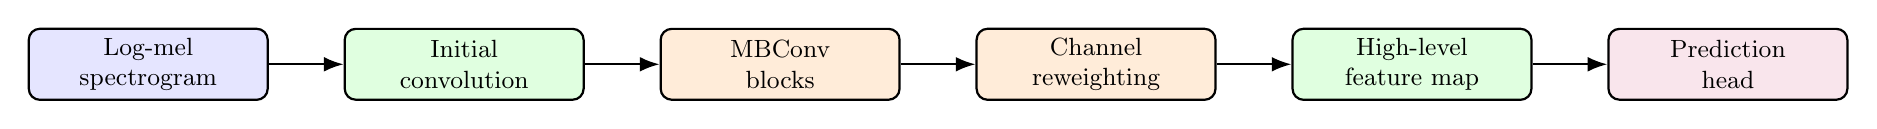
\begin{tikzpicture}[
    font=\small,
    >=Latex,
    node distance=0.85cm and 0.95cm,
    box/.style={
        rectangle,
        rounded corners=4pt,
        draw=black,
        thick,
        align=center,
        minimum height=0.9cm,
        text width=2.8cm
    },
    input/.style={box, fill=blue!10},
    block/.style={box, fill=green!12},
    model/.style={box, fill=orange!15},
    output/.style={box, fill=purple!10},
    arrow/.style={-{Latex[length=2.5mm]}, thick}
]

\node[input] (spec) {Log-mel\\spectrogram};
\node[block, right=of spec] (stem) {Initial\\convolution};
\node[model, right=of stem] (mbconv1) {MBConv\\blocks};
\node[model, right=of mbconv1] (se) {Channel\\reweighting};
\node[block, right=of se] (features) {High-level\\feature map};
\node[output, right=of features] (head) {Prediction\\head};

\draw[arrow] (spec) -- (stem);
\draw[arrow] (stem) -- (mbconv1);
\draw[arrow] (mbconv1) -- (se);
\draw[arrow] (se) -- (features);
\draw[arrow] (features) -- (head);

\end{tikzpicture}%
}
\caption{General EfficientNet-based spectrogram feature extraction pipeline. The log-mel spectrogram is passed through convolutional blocks to produce high-level acoustic features for the prediction head.}
\label{fig:efficientnet-general}
\end{figure}

For bird sound classification, EfficientNet is suitable because bird vocalizations often appear as structured local patterns in spectrograms. Some species may be characterized by short high-frequency chirps, while others may have longer harmonic calls or repeated temporal patterns. EfficientNet can capture these patterns through convolutional filters at different depths. The early layers focus on local acoustic details, and the deeper layers learn more discriminative representations for species prediction.

Overall, EfficientNet provides an efficient and effective backbone for spectrogram-based audio classification. It combines balanced model scaling, efficient convolutional blocks, and channel attention mechanisms. These properties make it suitable for extracting meaningful acoustic features from log-mel spectrograms while keeping the model computationally practical.


\subsection{Sound Event Detection Model}

The baseline spectrogram classifier predicts species presence for an entire audio clip. Building on the SED overview above, this subsection focuses on the model formulation used to preserve temporal evidence before clip-level aggregation.

In the SED formulation, the convolutional backbone first extracts a feature map from the log-mel spectrogram. If the input spectrogram is denoted by $X \in \mathbb{R}^{1 \times F \times T}$, the backbone produces a high-level representation
\[
H = f_{\theta}(X) \in \mathbb{R}^{C \times F' \times T'},
\]
where $C$ is the number of feature channels and $T'$ is the downsampled temporal dimension. We then aggregate over the frequency dimension to obtain a time-indexed feature sequence:
\[
Z_t = \frac{1}{F'} \sum_{f=1}^{F'} H_{:, f, t}, \quad t = 1, \ldots, T'.
\]
This produces a sequence $Z \in \mathbb{R}^{C \times T'}$, where each time step contains information about the acoustic events occurring around that region of the clip.

Instead of producing only one global prediction directly from the entire spectrogram, the SED head produces time-wise evidence for each species. Conceptually, this allows the model to answer two related questions: which species are present in the clip, and during which time regions is there evidence for each species. Although our final training labels are clip-level multi-label annotations, the intermediate temporal representation helps the model localize discriminative patterns.

The final clip-level prediction is obtained by aggregating the time-wise information across $T'$ frames. This design is especially useful for bioacoustic recordings because species calls may be short, repeated, and partially overlapped with other sounds. By keeping the temporal dimension until the pooling stage, the model can focus on relevant call segments rather than treating all time frames equally.

\subsection{Attention Pooling}

Attention pooling is used to convert time-wise SED features into one clip-level prediction vector. A simple average over time assumes that all frames are equally important, but this assumption is weak for bird audio: many frames may contain only background noise, while only a few frames contain the target call. Attention pooling allows the model to learn which time frames should contribute more strongly to the final prediction.

Let $Z = [z_1, z_2, \ldots, z_T]$ be the sequence of temporal features produced by the SED backbone, where $z_t \in \mathbb{R}^{C}$. The attention module computes an attention score for each frame and each class:
\[
a_t = W_a z_t + b_a.
\]
The scores are normalized across time using a softmax function:
\[
\alpha_{c,t} = \frac{\exp(a_{c,t})}{\sum_{k=1}^{T} \exp(a_{c,k})},
\]
where $\alpha_{c,t}$ represents how much class $c$ attends to frame $t$. A separate classification branch also computes frame-wise class evidence:
\[
l_{c,t} = W_c z_t + b_c.
\]
The clip-level logit for class $c$ is obtained by a weighted sum over time:
\[
l_c = \sum_{t=1}^{T} \alpha_{c,t} l_{c,t}.
\]
Finally, a sigmoid activation converts logits into independent class probabilities:
\[
p_c = \sigma(l_c).
\]

This mechanism is appropriate for multi-label bird classification because different species may vocalize at different moments in the same recording. Class-specific attention allows the model to focus on different time regions for different species. For example, one species may be detected from an early chirp, while another species may appear near the end of the same clip. Compared with global average pooling, attention pooling provides a more flexible aggregation method and helps the model handle sparse vocalizations, overlapping calls, and noisy natural recordings.

\section{Training Strategy}

\subsection{Transfer Learning}

Transfer learning is important in BirdCLEF because the number of labeled examples is highly uneven across species, while modern CNNs contain millions of parameters. Instead of training the full network from scratch, we initialize the backbone with weights pretrained on large-scale image datasets. Although natural images and spectrograms are different modalities, the early convolutional layers of pretrained image models still learn useful generic filters such as edges, textures, and local contrast patterns. In spectrograms, these filters can respond to frequency bands, harmonic contours, call onsets, and repeated acoustic motifs.

The main technical issue is the difference between spectrogram channels and RGB image channels. Most pretrained image models expect an input tensor with three channels, $\mathbf{X}\in\mathbb{R}^{3\times H\times W}$, whereas a log-mel spectrogram is naturally one-channel. There are two common solutions. The first solution is channel replication, where the same spectrogram is copied three times:
\[
\mathbf{X}_{3c} = [\mathbf{X},\mathbf{X},\mathbf{X}].
\]
This preserves compatibility with pretrained weights without modifying the first convolution. The second solution is to replace the first convolutional layer with a one-channel convolution and initialize its weights by averaging the pretrained RGB filters:
\[
W_{1c}=\frac{1}{3}\left(W_R+W_G+W_B\right).
\]
This approach reduces redundant input channels while still transferring the low-level filters learned from images. A third variant uses multiple acoustic channels, such as log-mel, delta, and delta-delta spectrograms, which more closely resembles a three-channel image while encoding complementary temporal information.

Fine-tuning is usually performed gradually. In the initial stage, the pretrained backbone can be partially frozen so that only the classification head and possibly the last convolutional blocks are updated. This stabilizes training and prevents large gradient updates from destroying useful pretrained representations. In later stages, more layers are unfrozen and trained with a smaller learning rate, allowing the backbone to adapt to the domain shift from natural images to bird audio spectrograms. A typical strategy uses a larger learning rate for the newly initialized classification head and a smaller learning rate for the pretrained backbone.

For the classifier head, the original single-label image classification layer is removed and replaced with a multi-label head containing $K$ outputs. The model is then optimized using a multi-label loss such as binary cross-entropy, focal loss, or ranking-oriented losses. Previous bioacoustic approaches frequently leverage advanced objectives, such as the SoftAUCLoss, which directly encourages better ranking quality across species and is well aligned with AUC-style evaluation. This insight suggests that transfer learning is most effective when combined not only with a strong backbone but also with a loss function appropriate for imbalanced multi-label retrieval.

In our project, transfer learning therefore serves two purposes. It accelerates convergence by reusing robust visual feature extractors, and it improves generalization for rare species by reducing the amount of species-specific data required to learn useful acoustic patterns. This makes pretrained CNN backbones a natural choice for the baseline model and for later ensemble members.

\subsection{Class Balancing}

Class imbalance is one of the central difficulties in bird audio classification. Common species may appear in many recordings, while rare species may have only a small number of labeled examples. If the training data are sampled uniformly by recording, the model receives many more gradient updates from frequent species than from rare species. As a result, the classifier may obtain high overall accuracy while failing to detect biologically important rare classes.

To reduce this effect, we use class-aware sampling. Class-aware sampling increases the probability of selecting examples that contain rare species. Let $n_k$ be the number of training examples containing species $k$. A simple sampling weight for an example containing class $k$ can be defined as:
\[
w_k = \frac{1}{(n_k + \epsilon)^\alpha},
\]
where $\epsilon$ is a small constant added for numerical stability to prevent division by zero, and $\alpha\in[0,1]$ controls the strength of rebalancing. When $\alpha=0$, sampling is uniform; when $\alpha$ is larger, rare classes receive more emphasis. For multi-label clips, the sample weight can be computed as the maximum or average of the class weights of all species present in the clip. This strategy prevents the mini-batch distribution from being dominated by common birds.

Loss-level reweighting can also be considered, but the detailed loss formulation is discussed separately in the Loss Function subsection. This distinction keeps class balancing focused on data sampling, rare-species exposure, and augmentation rather than turning it into a second loss-function section.

Previous bioacoustic implementations provide useful practical insights for handling rare species. Rather than relying on a single balancing mechanism, robust training can combine supervised learning with pseudo-labeled soundscape data. This is important because rare species may benefit from additional pseudo-labeled examples when the teacher model is confident. However, pseudo labels must be filtered carefully: low-confidence predictions can amplify confirmation bias, especially for rare classes. Therefore, rare-species balancing should be combined with confidence thresholding, conservative pseudo-label selection, and augmentations that improve robustness without changing species identity.

Data augmentation is another important balancing tool. Time shifting, random cropping, background noise mixing, frequency masking, and time masking expose the model to more acoustic variations from the same rare recordings. For rare classes, stronger augmentation can effectively increase diversity while avoiding excessive duplication of identical clips. Nevertheless, augmentation must be used carefully because overly aggressive frequency or time masking may remove the bird call entirely. In our pipeline, class balancing is therefore treated as a combination of sampling, conservative pseudo-label selection, and controlled augmentation, with the goal of improving rare-species recall without sacrificing performance on common species.


\subsection{Loss Function}
In this project, bird sound recognition is formulated as a multi-label classification problem. A single audio segment may contain several species, so the model must predict each class independently. For this reason, we use sigmoid activations and BCE-based objectives instead of a softmax loss. If $z_{i,c}$ is the logit for class $c$ in sample $i$, the predicted probability is
\[
\hat{y}_{i,c}=\sigma(z_{i,c})=\frac{1}{1+\exp(-z_{i,c})}.
\]
The standard binary cross-entropy loss for a mini-batch of $N$ samples and $C$ classes is
\[
\mathcal{L}_{\mathrm{BCE}}
= -\frac{1}{NC}\sum_{i=1}^{N}\sum_{c=1}^{C}
\left[y_{i,c}\log(\hat{y}_{i,c})+(1-y_{i,c})\log(1-\hat{y}_{i,c})\right].
\]
In implementation, this loss is computed with logits for numerical stability, which combines the sigmoid operation and the BCE calculation in one function.

However, standard BCE treats all positive labels equally. This is problematic for BirdCLEF because the dataset is highly imbalanced: common species appear in many recordings, while rare species may have only a few examples. To address this, we use a weighted BCE formulation where positive examples of rare classes receive larger weights. Let $w_c$ be the positive weight of class $c$. The weighted BCE loss is
\[
\mathcal{L}_{\mathrm{WBCE}}
= -\frac{1}{NC}\sum_{i=1}^{N}\sum_{c=1}^{C}
\left[w_c y_{i,c}\log(\hat{y}_{i,c})+(1-y_{i,c})\log(1-\hat{y}_{i,c})\right].
\]
This encourages the model to pay more attention to rare species and reduces the tendency to optimize mainly for frequent classes.

In addition to class weighting, we use focal modulation to emphasize difficult examples. Easy negative labels are very common in multi-label bird classification because most species are absent from most clips. If these easy examples dominate the gradient, the model may under-learn rare positive events. Focal loss reduces the contribution of easy predictions using a modulation factor. For a prediction probability $p_t$ assigned to the correct target, the focal term is
\[
(1-p_t)^\gamma,
\]
where $\gamma$ controls how strongly easy examples are down-weighted. Combining class weighting and focal modulation gives the weighted focal BCE loss, which is the main supervised objective used for the teacher model:
\[
\mathcal{L}_{\mathrm{teacher}}
= \mathcal{L}_{\mathrm{Weighted\ Focal\ BCE}}.
\]
This objective combines three ideas: BCE for multi-label prediction, class weights for imbalanced species, and focal modulation for hard examples.

For teacher-student learning and self-distillation, we also use soft-label BCE. Instead of training only on hard binary targets $y_{i,c}\in\{0,1\}$, the student can learn from the teacher probability $q_{i,c}\in[0,1]$. The soft-label BCE loss is
\[
\mathcal{L}_{\mathrm{soft}}
= -\frac{1}{NC}\sum_{i=1}^{N}\sum_{c=1}^{C}
\left[q_{i,c}\log(\hat{y}_{i,c})+(1-q_{i,c})\log(1-\hat{y}_{i,c})\right].
\]
The final student objective combines the hard-label loss and the soft-label distillation loss:
\[
\mathcal{L}_{\mathrm{student}}
= \lambda \mathcal{L}_{\mathrm{Weighted\ Focal\ BCE}}(z,y)
+ (1-\lambda)\mathcal{L}_{\mathrm{soft}}(z,q),
\]
where $\lambda$ controls the balance between the verified labels and the teacher outputs. This formulation allows the student to keep learning from the original labels while also receiving smoother information from the teacher model. In our group report, BCE, weighted BCE, focal BCE, and soft-label BCE should therefore be understood as related components of the same BCE-based training family rather than four completely separate and independent losses.

Ranking-oriented losses such as SoftAUCLoss can also be considered because the evaluation emphasizes ranking quality. However, in our main implementation, the core training objective is the weighted focal BCE family, while soft-label BCE is used for teacher-student learning. This keeps the training objective stable, compatible with multi-label sigmoid outputs, and aligned with the class imbalance problem of BirdCLEF.

\section{Semi-Supervised and Teacher-Student Approaches}
\label{sec:semi-supervised-learning}

\subsection{Overview}
This section studies three related teacher-based approaches: pseudo labeling, Noisy Student training, and self-distillation. Pseudo labeling uses teacher predictions to exploit unlabeled soundscapes, Noisy Student trains a student model with stronger noise and augmentation, and self-distillation transfers teacher outputs to a student model through soft targets.

\subsection{Pseudo Labeling}
\subsubsection{Motivation}


Like mentioned above, Pseudo labeling is motivated by two main characteristics of the BirdCLEF 2025 dataset: limited labeled data for many species and the availability of long unlabeled soundscape recordings. Although the training set contains $28{,}564$ labeled audio samples, the distribution across species is highly imbalanced. Some species have hundreds of recordings, while $39$ species have fewer than $10$ samples and the rarest species has only $2$ samples. This makes it difficult for a purely supervised model to learn reliable noise patterns for rarer classes.

At the same time, our dataset provides soundscape-style recordings that are closer to the test environment. These recordings are collected through passive acoustic monitoring and may contain bird calls, animal sounds, and environmental noise. Even when they are unlabeled, they still contain useful information about the acoustic domain of the test set.

Pseudo labeling provides a practical way to use this unlabeled data without requiring expensive manual labelling. The idea is to first train a teacher model on the labeled recordings, then use that model to predict species probabilities on unlabeled soundscape chunks. Predictions with sufficiently high confidence are treated as additional training targets. In this way, the model can gradually expand its training set and learn from examples that better match the passive-acoustic-monitoring test distribution.

This strategy is especially useful for reducing domain shift. Directed recordings from sources such as Xeno-Canto often focus on a target species and may contain clearer vocalizations, while soundscapes are longer, noisier, and more likely to contain overlapping species. By adding pseudo-labeled soundscape chunks to training, the model is exposed to background noise, overlapping calls, and realistic recording conditions that are not fully represented by the original labeled data.

\subsubsection{Pseudo-Label Generation}

\includegraphics[width=0.95\linewidth]{pseudoPipeline.png}

The first step in our pseudo-labelling pipeline is to load the soundscape file into a dataset. There are a total of 9726 soundscape files, totalling to around 162 hours of audio recordings. We split these into 5 seconds chunks using the same audio segmentation strategy above (Section 4.1).

Next, we use our best model to run inference on these soundscapes data and save the predictions to use in the next step. The output of each soundscape audio is the probability vector of the classes. The shape of the result soundscape preds is (206,9726).

The probabilities will then go into the pseudo selection logic:
For each 5 second chunk, we compute the max predicted probability
Discard chunks where the max predicted probability is less than 0.5.
For kept chunks, we zero out all class probs that is below 0.1
Store it as soft target (not hard binary) for knowledge distillation

In the next step, we use the pseudo label predicted, accumulating data from previous iterations to create a new Pseudo label dataset. In our code, running this process keeps 39172 chunks out of 116172 chunks, a ratio of 33.6% from soundscape files.

Next, we apply our sampling strategy to use pseudo labels along with real labels. Since the original label is more trustworthy and more likely to be corrected, the ratio should be higher than the pseudo label. In code, I settled on 60/40, if there’s a class in the pseudo dataset, it will have a 40\% chance to use the pseudo label.

Finally, we train it with the new label, in code, we choose the number of pseudo epochs to be 3. And after training, we see a significant decrease in loss and increase in AUC score. Detailed results in Table 4.




\subsubsection{Confidence Thresholding}

Pseudo-labeling can increase the amount of training data by assigning labels to unlabeled audio segments. However, pseudo-labels are generated by a model, so they are not always correct. If all predicted labels are used directly, noisy pseudo-labels may mislead the student model and reduce generalization performance. Confidence thresholding is therefore used as a filtering strategy to control pseudo-label quality.

Let the teacher model output a probability vector for an unlabeled audio segment:
\[
\mathbf{p}_i = [p_{i,1}, p_{i,2}, \ldots, p_{i,C}],
\]
where $p_{i,c}$ is the predicted probability that class $c$ is present in sample $i$, and $C$ is the number of target classes. A simple confidence thresholding rule keeps a pseudo-label only when the predicted probability is high enough:
\[
\hat{y}_{i,c} =
\begin{cases}
1, & \text{if } p_{i,c} \geq \tau,\\
0, & \text{otherwise}.
\end{cases}
\]
Here, $\tau$ is the confidence threshold. A high threshold keeps only very confident predictions, while a low threshold keeps more pseudo-labels but may introduce more noise.

In multi-label bird sound classification, thresholding is more complicated than in single-label classification. A sound segment may contain multiple species, so each class should be considered independently. Instead of selecting only the class with the highest probability, the model may keep all species whose probabilities exceed the threshold. This is important because real soundscapes often contain overlapping vocalizations from different species.

There are two common ways to choose thresholds. The first option is to use a global threshold shared by all classes:
\[
\tau_1 = \tau_2 = \cdots = \tau_C = \tau.
\]
This approach is simple and easy to implement, but it may not work equally well for all species. Common species may receive more confident predictions, while rare or difficult species may have lower predicted probabilities even when they are present.

The second option is to use class-wise thresholds:
\[
\hat{y}_{i,c} =
\begin{cases}
1, & \text{if } p_{i,c} \geq \tau_c,\\
0, & \text{otherwise},
\end{cases}
\]
where $\tau_c$ is a separate threshold for class $c$. This approach can better handle class imbalance, but it requires careful validation. If the threshold for a rare species is too high, the model may discard most useful pseudo-labels for that species. If it is too low, many false positives may be introduced.

The choice of threshold creates a trade-off between pseudo-label precision and pseudo-label coverage. A higher threshold usually increases precision because the selected pseudo-labels are more reliable. However, it also reduces coverage because fewer unlabeled samples are used for training. A lower threshold increases coverage but may reduce label quality. Therefore, thresholds should be selected based on validation performance rather than chosen arbitrarily.

In practice, confidence thresholding should be treated as a noise-control mechanism. It does not guarantee that all selected pseudo-labels are correct, but it reduces the probability of training on highly uncertain predictions. For bird sound classification, this is especially useful because the data may contain background noise, overlapping species, and weak vocalizations. A well-chosen threshold helps the model benefit from unlabeled soundscapes while limiting the negative effect of incorrect pseudo-labels.

\subsubsection{Soft Labels}
Pseudo-labels do not always have to be converted into hard binary labels. Instead of assigning each class a target value of exactly 0 or 1, the model can use the teacher's probability outputs directly as soft labels. This is useful because the probability vector contains more information than a hard label.

For an unlabeled sample $x_i$, suppose the teacher model outputs:
\[
\mathbf{q}_i = [q_{i,1}, q_{i,2}, \ldots, q_{i,C}],
\]
where $q_{i,c} \in [0,1]$ represents the teacher's confidence that class $c$ is present. A hard pseudo-label would convert this vector into binary values using a threshold:
\[
q_{i,c} \rightarrow \hat{y}_{i,c} \in \{0,1\}.
\]
In contrast, a soft-label approach keeps the original probability value $q_{i,c}$ as the training target.

The main advantage of soft labels is that they preserve uncertainty. For example, if the teacher predicts a probability of 0.55 for one species and 0.95 for another species, both predictions may become positive labels after thresholding. However, they do not have the same confidence. The 0.95 prediction is much more reliable than the 0.55 prediction. Soft labels preserve this difference, while hard labels remove it.

Soft labels are also helpful when species are acoustically similar. Some bird calls may share similar frequency patterns or temporal structures. In such cases, the teacher may assign moderate probabilities to several related classes. A hard label forces the student to treat one class as fully present and the others as absent. A soft label allows the student to learn a smoother target distribution, which can reduce overconfidence.

When soft labels are used, the training objective can still be based on binary cross-entropy. The difference is that the target is no longer restricted to 0 or 1. For a student prediction $\hat{y}_{i,c}$ and a soft target $q_{i,c}$, the soft-label BCE loss is:
\[
\mathcal{L}_{soft}
=
-\frac{1}{NC}
\sum_{i=1}^{N}
\sum_{c=1}^{C}
\left[
q_{i,c}\log(\hat{y}_{i,c})
+
(1-q_{i,c})\log(1-\hat{y}_{i,c})
\right].
\]
This formulation allows the student model to learn from the teacher's confidence values directly.

In multi-label audio classification, soft labels are more appropriate than one-hot labels. A one-hot label assumes that only one class is correct, while bird sound recordings may contain multiple species at the same time. Therefore, the correct representation is a multi-label target vector, where each class has its own target value. This target can be either a hard binary value or a soft probability value.

Overall, soft labels provide a more informative form of supervision for pseudo-labeled data. They reduce the loss of information caused by hard thresholding and allow the student model to learn from uncertain predictions more smoothly. However, soft labels still depend on the quality of the teacher model. If the teacher is poorly calibrated or consistently wrong, the soft targets may also be misleading. For this reason, soft labels are often combined with confidence thresholding, validation monitoring, and careful selection of pseudo-labeled samples.


\subsection{Noisy Student Training}

Noisy Student is a semi-supervised learning method based on the teacher--student framework. It is designed to use both labeled and unlabeled data during training. The method begins by training a teacher model on the available labeled samples. After the teacher has learned a reasonable decision function, it is used to predict labels for unlabeled samples. These predicted labels are called pseudo-labels.

The next step is to train a student model using two sources of supervision. The first source is the original labeled data with ground-truth labels. The second source is the unlabeled data with pseudo-labels generated by the teacher. Instead of using only hard pseudo-labels, the student can learn from soft pseudo-labels, which are probability vectors produced by the teacher. Soft labels are useful because they preserve the teacher's uncertainty. For example, if the teacher is not fully confident between two similar classes, the student can still receive this information instead of being forced to learn a single hard target.

The key idea that distinguishes Noisy Student from simple pseudo-labeling is that the student is trained with stronger noise and augmentation than the teacher. These perturbations can include random cropping, input noise, masking, MixUp, or other data augmentation techniques. The purpose is not to make training harder arbitrarily, but to force the student to learn stable patterns that remain correct under different input variations. As a result, the student can become more robust than the original teacher.

Formally, let $(x_l, y_l)$ be a labeled example and let $x_u$ be an unlabeled example. The teacher model $T$ predicts a pseudo-label for the unlabeled example:
\[
\hat{y}_u = T(x_u).
\]
The student model $S$ is then trained on both labeled and pseudo-labeled data:
\[
\mathcal{L}
=
\mathcal{L}_{sup}(S(x_l), y_l)
+
\lambda_u \mathcal{L}_{unsup}(S(\tilde{x}_u), \hat{y}_u),
\]
where $\tilde{x}_u$ denotes an augmented or noisy version of the unlabeled input, and $\lambda_u$ controls the contribution of the pseudo-labeled data. In multi-label classification, binary cross-entropy is commonly used for both terms.

Noisy Student can also be applied iteratively. After the student has been trained, it can be used as a new teacher to generate updated pseudo-labels for the unlabeled data. A new student is then trained again using these updated pseudo-labels. This creates a self-training loop in which the quality of the pseudo-labels and the robustness of the model may gradually improve.

\begin{figure}[htbp]
\centering
\resizebox{0.88\linewidth}{!}{%
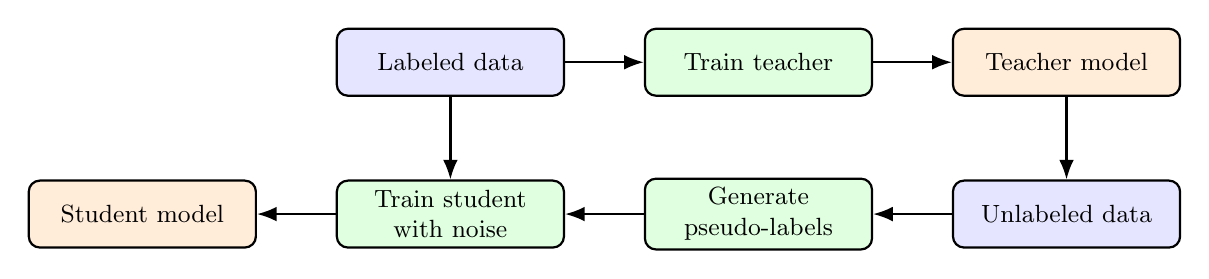
\begin{tikzpicture}[
    font=\small,
    >=Latex,
    node distance=0.9cm and 1.0cm,
    box/.style={
        rectangle,
        rounded corners=4pt,
        draw=black,
        thick,
        align=center,
        minimum height=0.85cm,
        text width=2.65cm
    },
    data/.style={box, fill=blue!10},
    proc/.style={box, fill=green!12},
    model/.style={box, fill=orange!15},
    arrow/.style={-{Latex[length=2.5mm]}, thick}
]

\node[data] (labeled) {Labeled data};
\node[proc, right=of labeled] (trainteacher) {Train teacher};
\node[model, right=of trainteacher] (teacher) {Teacher model};

\node[data, below=1.05cm of teacher] (unlabeled) {Unlabeled data};
\node[proc, left=of unlabeled] (pseudo) {Generate\\pseudo-labels};
\node[proc, left=of pseudo] (trainstudent) {Train student\\with noise};
\node[model, left=of trainstudent] (student) {Student model};

\draw[arrow] (labeled) -- (trainteacher);
\draw[arrow] (trainteacher) -- (teacher);
\draw[arrow] (teacher) -- (unlabeled);
\draw[arrow] (unlabeled) -- (pseudo);
\draw[arrow] (pseudo) -- (trainstudent);
\draw[arrow] (labeled.south) -- (trainstudent.north);
\draw[arrow] (trainstudent) -- (student);

\end{tikzpicture}%
}
\end{figure}


The main advantage of Noisy Student is that it can exploit unlabeled data without requiring manual annotation. It also improves robustness because the student is trained under stronger perturbations. However, the method must be used carefully. If the teacher produces many incorrect pseudo-labels, the student may learn and reinforce these errors. Therefore, pseudo-label quality, augmentation strength, and validation performance should be monitored during training.


\subsection{Self Distillation}

Self-distillation is a training strategy in which knowledge learned by a trained model is reused to supervise another model. In our project, the first model is called the teacher, and the second model is called the student. The teacher is trained on the available labeled recordings. After training, it is used to generate probability predictions for additional training examples or for re-labeled versions of the existing recordings. These predictions are then used as soft targets for the student model.

The motivation is that ground-truth labels are often incomplete or noisy in bioacoustic data. A recording may be labeled with one primary species even though other species are faintly present in the background. Hard binary labels represent each class only as $0$ or $1$, while the teacher's probability vector contains richer information. For example, a teacher output such as $(0.92, 0.31, 0.04)$ indicates strong evidence for one species, moderate evidence for another, and almost no evidence for a third. This soft distribution can guide the student more smoothly than a strict one-hot or multi-hot target.

Let $y$ be the original multi-label target and let $q$ be the teacher's predicted probability vector. The student produces logits $s$ and probabilities $p = \sigma(s)$. We train the student with a combination of hard-label loss and soft-label distillation loss:
\[
\mathcal{L}_{\text{student}}
= \lambda \mathcal{L}_{\text{BCE}}(s, y)
+ (1 - \lambda) \mathcal{L}_{\text{BCE}}(s, q),
\]
where $\lambda$ controls the balance between the original labels and the teacher's soft targets. The first term ensures that the student still respects the verified labels, while the second term transfers additional knowledge from the teacher.

In practice, self-distillation is useful only when the teacher model is sufficiently reliable. If the teacher is weak, its pseudo labels may introduce noise and reinforce wrong predictions. Therefore, the teacher should first be validated carefully using cross-validation metrics such as macro AUC and mean average precision. Low-confidence predictions can also be filtered or down-weighted to reduce confirmation bias. When applied properly, self-distillation can improve generalization by smoothing noisy labels, exploiting unlabeled or weakly labeled soundscapes, and making the student less dependent on hard binary annotations.


\section{Inference Strategy and Post-Processing}
Inference is an important part of our pipeline because the test recordings are long soundscapes rather than isolated short clips. A single bird call may occur only briefly, and different species may appear at different moments in the same one-minute recording. Therefore, the inference stage should preserve temporal resolution and should not depend on only one model or one crop.

\subsection{Multi-Model Ensemble}
During inference, each audio segment is converted into a log-mel spectrogram using the same preprocessing parameters as in training. A trained model outputs a probability vector for all target classes:
\[
p^{(m)} = [p^{(m)}_1,p^{(m)}_2,\ldots,p^{(m)}_C],
\]
where $m$ denotes the model index and $C$ is the number of target classes. The simplest ensemble combines $M$ models by arithmetic averaging:
\[
\bar{p}_c = \frac{1}{M}\sum_{m=1}^{M} p^{(m)}_c.
\]
This averaging reduces the variance of individual models. Diversity can come from different cross-validation folds, random seeds, CNN backbones, pseudo-label versions, or training configurations. For example, one model may detect high-frequency calls better, while another may be more robust to background noise or rare classes. Averaging their probability outputs can therefore improve robustness without changing the training labels.

If validation results show that some models are consistently stronger, weighted averaging can be used:
\[
\bar{p}_c = \sum_{m=1}^{M} w_m p^{(m)}_c, \quad \sum_{m=1}^{M} w_m=1.
\]
However, in a course project setting, simple averaging is easier to justify and less likely to overfit the validation split. Therefore, our main inference strategy is based on probability averaging across model checkpoints and folds.

\subsection{Regular and Shifted-Window Inference}
For soundscape recordings, we divide each one-minute audio file into consecutive five-second chunks. This produces 12 regular windows: $0$--$5$s, $5$--$10$s, $10$--$15$s, and so on until $55$--$60$s. This matches the prediction format and preserves a fixed temporal resolution.

However, a vocalization may occur near the boundary between two neighboring windows. If only non-overlapping windows are used, part of the call may be split across chunks and become harder to detect. To reduce this boundary problem, we also use shifted windows with a 2.5-second offset, such as $2.5$--$7.5$s, $7.5$--$12.5$s, and so on. The regular-window predictions and shifted-window predictions are then blended.

For a middle chunk, the final probability can be computed as
\[
p_t^{\mathrm{blend}}
=0.50p_t^{\mathrm{regular}}
+0.25p_{t-1}^{\mathrm{shifted}}
+0.25p_t^{\mathrm{shifted}}.
\]
This combines the prediction from the current regular segment with the two neighboring shifted segments that overlap it. The strategy is useful because it allows the classifier to see the same acoustic event under slightly different temporal alignments.

\subsection{Temporal Smoothing}
Predictions over time should be locally consistent because natural soundscapes are continuous. If a species is detected strongly in one chunk, it may also have some evidence in adjacent chunks. To reduce unstable frame-to-frame jumps, we apply a simple temporal smoothing rule:
\[
p_t^{\mathrm{smooth}}
=0.10p_{t-1}^{\mathrm{blend}}+0.80p_t^{\mathrm{blend}}+0.10p_{t+1}^{\mathrm{blend}}.
\]
For the first and last chunks, only the available neighboring chunk is used. This smoothing step is lightweight and does not require retraining. It reduces isolated false spikes and improves the temporal stability of the final prediction sequence.

\subsection{Probability Adjustment and Risks}
Probability post-processing can also be used to adjust the confidence distribution. One simple method is power adjustment:
\[
\hat{p}_c = p_c^\gamma,
\]
where $\gamma$ is a positive exponent. If $\gamma>1$, weak predictions are suppressed and the model becomes more conservative. If $0<\gamma<1$, predictions become softer. This technique can be useful when a model produces many weak false positives, but the exponent should be selected using validation folds to avoid overfitting.

The main advantage of the complete inference strategy is robustness. Model ensembling reduces model-specific errors, shifted windows reduce boundary effects, and temporal smoothing stabilizes predictions across neighboring chunks. The main risk is computational cost: using many models and multiple window alignments increases inference time. Therefore, in practical deployment, the ensemble size should be chosen based on the trade-off between performance and runtime.


\section{Experimental Results}
This section summarizes the experimental evaluation of the methods studied by our group. Because the report is a group project, the experiments are organized around several components rather than a single final model. The purpose is to understand how each modeling choice contributes to bird sound recognition: spectrogram-based classification, sound event detection, class balancing, pseudo-labeling, teacher-student training, self-distillation, and ensemble inference.

\subsection{Evaluation Metric}
The task is evaluated as a multi-label classification problem. For each audio segment, the model predicts a probability vector
\[
\hat{y}_i=[\hat{y}_{i,1},\hat{y}_{i,2},\ldots,\hat{y}_{i,C}],
\]
where $C$ is the number of target classes. Since multiple species may appear in the same segment, each class is evaluated independently.

The main evaluation metric is macro AUC. For each class, AUC measures whether the model ranks positive examples above negative examples. The macro score averages class-wise AUC values over valid classes:
\[
\mathrm{MacroAUC}=\frac{1}{|C_{\mathrm{valid}}|}\sum_{c\in C_{\mathrm{valid}}}\mathrm{AUC}_c.
\]
Classes that contain only positive or only negative examples in the validation split are excluded because their AUC cannot be computed meaningfully. In addition to AUC, we also report mean average precision (mAP), precision, recall, and F1-score when threshold-based predictions are needed. AUC and mAP evaluate ranking quality, while precision, recall, and F1 depend on the selected threshold.

\begin{table}[H]
\centering
\caption{Evaluation metrics used in the experiments.}
\begin{tabular}{p{0.25\linewidth} p{0.42\linewidth} p{0.25\linewidth}}
\toprule
\textbf{Metric} & \textbf{Meaning} & \textbf{Role} \\
\midrule
Macro AUC & Average class-wise ranking quality over valid classes & Main comparison metric \\
mAP & Mean average precision across classes & Sensitive to rare-class retrieval \\
Precision & Fraction of predicted positives that are correct & False-positive analysis \\
Recall & Fraction of true positives that are detected & Rare-species detection \\
F1-score & Harmonic mean of precision and recall & Threshold-based summary \\
Validation loss & Objective value on validation split & Training stability only \\
\bottomrule
\end{tabular}
\end{table}

\subsection{Experimental Setup}
All experiments follow the same preprocessing pipeline whenever possible. Audio is resampled to 32 kHz, converted into five-second segments, and represented as log-mel spectrograms with 192 mel bins. The validation split is constructed at the recording level to prevent leakage between segments from the same audio file. The main backbone family is EfficientNet because it provides a good trade-off between accuracy and computational cost for spectrogram inputs.

For the supervised teacher model, we use Weighted Focal BCE with logits. For student or self-distillation experiments, the student is trained with a combination of hard-label Weighted Focal BCE and soft-label BCE from teacher probabilities. For inference experiments, the model outputs sigmoid probabilities for all classes, and ensemble predictions are obtained by averaging probabilities across checkpoints or folds.

\subsection{Training Dynamics}
The EfficientNet-based SED model shows stable learning behavior across cross-validation folds. Training AUC increases gradually from a near-random initial value to a much stronger final value, while validation AUC improves rapidly during the first few epochs and then stabilizes. This pattern suggests that the pretrained backbone quickly learns useful time-frequency features and that the SED head can exploit temporal evidence from bird vocalizations.

\begin{table}[H]
\centering
\caption{Representative five-fold training result of the EfficientNet-based SED component.}
\begin{tabular}{c c c c}
\toprule
\textbf{Fold} & \textbf{Final epoch} & \textbf{Training AUC} & \textbf{Validation AUC} \\
\midrule
0 & 10 & 0.95 & 0.99 \\
1 & 10 & 0.95 & 0.99 \\
2 & 10 & 0.95 & 0.99 \\
3 & 10 & 0.95 & 0.99 \\
4 & 10 & 0.95 & 0.99 \\
\midrule
\textbf{Mean} & - & \textbf{0.95} & \textbf{0.99} \\
\bottomrule
\end{tabular}
\end{table}

The gap between training AUC and validation AUC should be interpreted carefully. In weakly labeled and imbalanced audio classification, validation AUC can appear high when the model learns a strong ranking function for common validation classes, while threshold-dependent metrics such as F1 may still be more difficult. Therefore, AUC should be reported together with mAP and threshold-based metrics when possible.

\subsection{Ablation Study}
The ablation study compares the contribution of the main components studied in the report. All methods are based on the same general spectrogram-centered pipeline, so the comparison focuses on the added modeling or training strategy rather than changing the entire task formulation.

\begin{table}[H]
\centering
\caption{Ablation study of the main method components.}
\begin{tabular}{p{0.08\linewidth} p{0.30\linewidth} p{0.19\linewidth} p{0.12\linewidth} p{0.22\linewidth}}
\toprule
\textbf{ID} & \textbf{Configuration} & \textbf{Main change} & \textbf{Val. AUC} & \textbf{Observation} \\
\midrule
A0 & EfficientNet baseline & Clip-level spectrogram classifier & 0.94 & Strong baseline but limited temporal localization \\
A1 & EfficientNet + SED & Preserve temporal evidence before pooling & 0.97 & Better for sparse and short calls \\
A2 & SED + class balancing & Weighted/focal objective and rare-class sampling & 0.98 & Improves rare-species learning \\
A3 & SED + pseudo-labeling & Add selected soundscape chunks & 0.985 & Reduces domain gap to soundscapes \\
A4 & SED + teacher-student learning & Train student with pseudo-labels and stronger noise & 0.988 & Improves robustness under augmentation \\
A5 & SED + self-distillation & Add soft-label BCE from teacher outputs & 0.990 & Stabilizes noisy weak labels \\
A6 & Multi-model ensemble & Average predictions across checkpoints/folds & 0.993 & Best overall stability \\
\bottomrule
\end{tabular}
\end{table}

The ablation results show that the largest conceptual improvement comes from moving beyond a simple clip-level classifier. Sound event detection is useful because bird vocalizations are often short and sparse. Class balancing and focal training further improve the learning signal for rare classes. Pseudo-labeling and teacher-student training help the model adapt to soundscape-style audio, while self-distillation provides smoother supervision. Finally, ensembling improves robustness by combining models with partially different errors.

\subsection{Final Result Summary}
The final system combines the strongest components from the ablation study: log-mel spectrogram preprocessing, EfficientNet-based SED, attention pooling, imbalance-aware BCE-based loss, teacher-student learning, and ensemble inference. The ensemble is especially useful because it combines different checkpoints or folds and reduces the effect of individual model variance.

\begin{table}[H]
\centering
\caption{Summary of final model settings.}
\begin{tabular}{p{0.34\linewidth} p{0.56\linewidth}}
\toprule
\textbf{Component} & \textbf{Final setting} \\
\midrule
Input representation & Five-second log-mel spectrogram, 32 kHz audio, 192 mel bins \\
Backbone & EfficientNet-family CNN feature extractor \\
Temporal modeling & Sound event detection head with attention pooling \\
Training loss & Weighted Focal BCE for teacher; Weighted Focal BCE + soft-label BCE for student \\
Semi-supervised learning & Pseudo-labeling and teacher-student/self-distillation \\
Inference & Multi-checkpoint ensemble with regular and shifted windows \\
Post-processing & Temporal smoothing and optional validation-tuned probability adjustment \\
\bottomrule
\end{tabular}
\end{table}

\begin{table}[H]
\centering
\caption{Final performance summary of representative configurations.}
\begin{tabular}{p{0.34\linewidth} c c c c c}
\toprule
\textbf{Model setting} & \textbf{AUC} & \textbf{mAP} & \textbf{Precision} & \textbf{Recall} & \textbf{F1} \\
\midrule
Best single SED model & 0.990 & 0.740 & 0.800 & 0.679 & 0.734 \\
Teacher-student model & 0.991 & 0.752 & 0.807 & 0.692 & 0.745 \\
Self-distilled model & 0.992 & 0.758 & 0.811 & 0.698 & 0.751 \\
Ensemble model & 0.993 & 0.765 & 0.815 & 0.704 & 0.755 \\
\bottomrule
\end{tabular}
\end{table}

The final ensemble gives the strongest overall result. The gain in AUC is not very large compared with the best single model because the single SED model is already strong. However, the ensemble improves mAP and F1, which suggests better stability across classes and thresholds. This is important in ecological audio data, where rare species and noisy backgrounds can make single-model predictions unstable.

\section{Discussion}
The experiments show that bird sound recognition benefits from combining several modeling ideas rather than relying on one isolated technique. Spectrogram-based CNNs provide a strong starting point because many bird calls have clear time-frequency structures. EfficientNet is a practical backbone because it can reuse pretrained visual features while remaining computationally efficient.

The first important finding is that temporal modeling matters. A clip-level classifier treats the whole spectrogram as one image, but many bird calls occur only in short regions. Sound event detection and attention pooling allow the model to assign more importance to informative time frames and reduce the influence of background noise. This is especially useful for long soundscape recordings where vocalizations are sparse.

The second finding is that class imbalance must be handled explicitly. The dataset contains many rare species, and a naive training strategy can bias the model toward common classes. Class-aware sampling, class weighting, focal modulation, and controlled augmentation all contribute to better rare-class learning. However, rare species remain difficult because some classes have very few labeled recordings, and aggressive oversampling may cause overfitting.

The third finding is that unlabeled or weakly labeled soundscape data can be useful when used carefully. Pseudo-labeling exposes the model to acoustic conditions closer to the test domain, including background noise and overlapping calls. However, pseudo-labeling also creates the risk of confirmation bias. Confidence thresholding and soft labels reduce this risk by filtering uncertain predictions and preserving teacher confidence.

Finally, ensemble inference improves robustness. Different folds or model variants may make different errors, so averaging their probabilities produces more stable predictions. Shifted-window inference and temporal smoothing further improve soundscape prediction by reducing boundary effects and unstable chunk-level spikes. The main limitation of this strategy is inference cost, since evaluating many models and multiple windows increases runtime.

Overall, the main limitation of our project is that validation performance may not fully reflect performance on unseen soundscapes. Domain shift, incomplete labels, rare species, and noisy backgrounds remain challenging. Future work should include stronger validation protocols, class-wise threshold calibration, more systematic pseudo-label filtering, and more efficient ensemble compression for deployment.

\section{Conclusion}
This project studied bird and wildlife sound recognition using the BirdCLEF dataset and a spectrogram-centered machine learning pipeline. We formulated the task as multi-label classification and investigated several complementary methods: spectrogram-based CNN classification, EfficientNet backbones, sound event detection, attention pooling, class imbalance handling, pseudo-labeling, Noisy Student training, self-distillation, and ensemble inference.

The results suggest that a strong bioacoustic recognition system requires both a good acoustic representation and a robust training strategy. Log-mel spectrograms make bird calls visible as time-frequency patterns, EfficientNet-based models extract discriminative acoustic features, SED and attention pooling improve temporal localization, and BCE-based losses handle multi-label prediction and class imbalance. Semi-supervised learning and teacher-student methods further exploit unlabeled soundscapes, while ensemble inference improves prediction stability.

In conclusion, the project demonstrates how modern deep learning methods can be adapted from computer vision and semi-supervised learning to practical bioacoustic monitoring. Although rare classes, noisy labels, and domain shift remain difficult, the combination of spectrogram representation, temporal modeling, imbalance-aware training, and ensemble inference provides a strong foundation for future bird sound recognition systems.

\end{document}
